{\setlength{\chapterfontsize}{23pt}
\chapter{Web service implementations}
}

\section{Data structures}
In this section, we describe the data structures used in our implementation. We cover the data contained in LameDuck and NiceView, followed by the more advanced BPEL and REST implementations.

\subsection{LameDuck}
LameDuck implement the data as described in the project description. To store this, we save all \texttt{FlightInformation} both as lists of \texttt{FlightInformation}s with the same origin airport and store a link from the \texttt{BookingNo} to the matching \texttt{Flight Information}. This is done to make look-ups easier to perform. It does add some extra bookkeeping at initialization of the data, but this is worth it to save complexity later on. The overall data structure is shown in Fig.~\ref{fig:lameduck_class}

\begin{figure}[H]
\centering
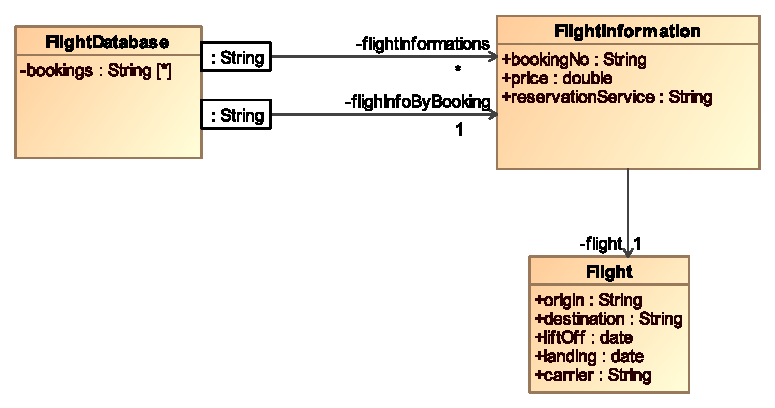
\includegraphics[width=0.8\textwidth]{LameDuck}
\caption{Data model of LameDuck}
\label{fig:lameduck_class}
\end{figure}


\subsection{NiceView}
\begin{figure}[H]
\centering
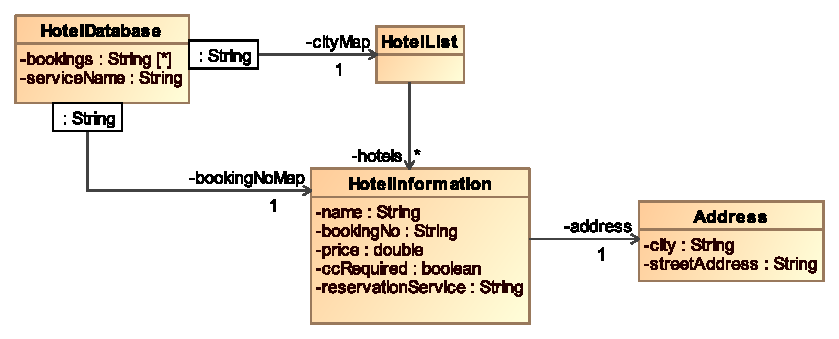
\includegraphics[width=0.8\textwidth]{NiceView}
\caption{Data model of NiceView}
\label{fig:niceview_class}
\end{figure}

\subsection{TravelGood - BPEL}
\todo{BPEL klasse diagram}

\subsection{TravelGood - RESTful}
The RESTful version of TravelGood uses the data structures shown in figure~\ref{fig:rest_class}. A \texttt{Customer} represents the user of a system. All customers are contained in the \texttt{CustomerDatabase}. This is done in a map where the key is the identifier of the customer. This is done so a customer can be found quickly. Each \texttt{Customer} can be connected with itineraries. This is handled in \texttt{ItineraryDatabase}. The \texttt{ItineraryDatabase} holds all the itineraries in a map where the identifier of the itinerary is the key in order to quickly look up an itinerary. An \texttt{Itinerary} contains a \texttt{FlightBookingList} and a \texttt{HotelBookingList} to keep track of \texttt{FlightBooking}s and \texttt{HotelBooking}s respectively.

\todo{REST klasse diagram}

\begin{figure}[H]
\centering
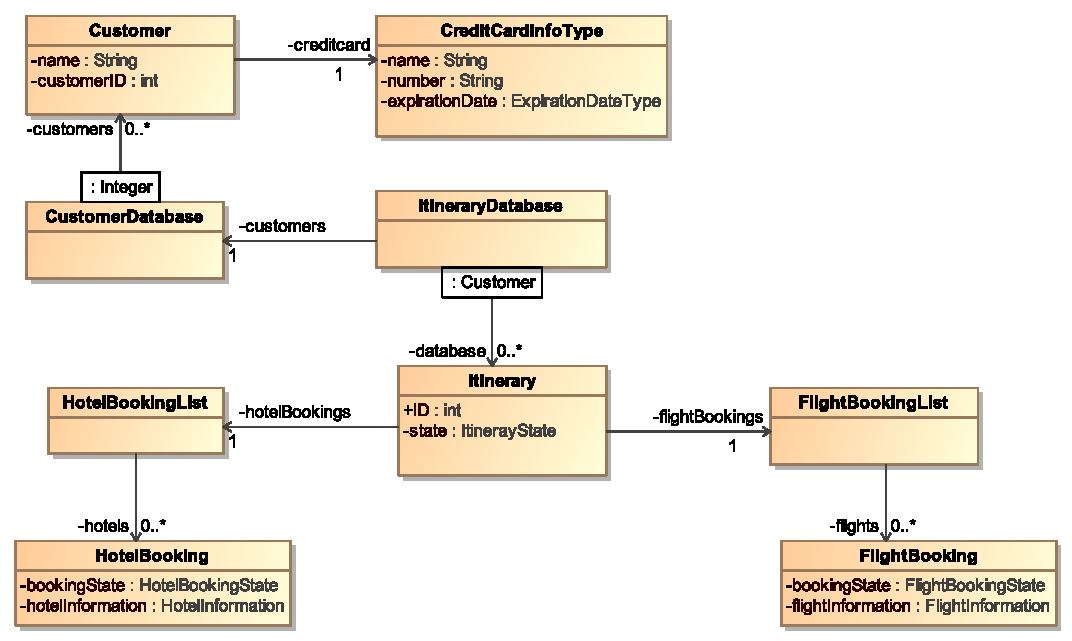
\includegraphics[width=0.8\textwidth]{TravelGoodREST}
\caption{Data model of TravelGoodREST}
\label{fig:rest_class}
\end{figure}


\section{Airline- and hotel services}
Both LameDuck and NiceView are implemented using RPC-Literal style, which has been done for the simplicity of the format. We do miss out on good things from the document style binding, such as reduced overhead in the SOAP message as well as the ability to validate the SOAP message -- we simply assume that the messages are formatted correctly. 
Also, following the rationale from \cite{papazoglou2008web}, this implementation is a synchronous service with parameter passing rather than an asynchronous document passing service.
\todo{Vi bør have en bedre grund til at vi ikke bruger Document style. Er denne ok? (KRC)}

For both services, we have developed a small suite of unit tests, that can be used to ensure that both services are implemented correctly, before running tests for the BPEL/RESTful implementations. For this purpose, we have added a service along with the required one, to reset the databases for the services.

The databases for each service is a small example with only a few entries that have been hard-coded in to suit the needs we have for our unit tests. An actual implementation of these would be much more complex, i.e. booking numbers are generated on a per-user basis and not just stored directly in the database.

\subsection{LameDuck}
The LameDuck service has been implemented with a wrapper class that implements the web service related things. The actual data is stored in a hard coded database, which is initialized by the web service class. This way we separate the business logic of communicating with the world from the business logic of maintaining the flights and the bookings. The web service class is also responsible for communicating with the bank when necessary, separating handling of money from handling flights.

We have created some hardcoded test data, which can be reset using a separate web service, that should only be used during testing. As such this web service is implemented with a separate WSDL. To allow both services to access the database, it has been implemented as a singleton object.


\subsection{NiceView}
The NiceView service has been implemented similarly to that of our LameDuck service, just with hotels instead of flights.

It also has a separate reset service from which one can reset our database to the initial state.


